\usepackage{hyperref}\newpage
\begin{center}
  \textbf{\large 2. ВЫБОР ТЕХНОЛОГИЙ И ПРОЕКТИРОВАНИЕ АИС}
\end{center}
\refstepcounter{chapter}
\addcontentsline{toc}{chapter}{2. ВЫБОР ТЕХНОЛОГИЙ И ПРОЕКТИРОВАНИЕ АИС}


\section{Анализ компонентов системы и требований к ним}
АИС "МТУСИ Расписание" включает следующие компоненты: 
\begin{enumerate}
  \item Мобильное приложение для просмотра расписания.
  \item Парсер для сбора и обработки данных расписания.
  \item API для доступа к данным расписания.
  \item ICS API для экспорта расписания в формате iCalendar.
\end{enumerate}


\subsection{Мобильное приложение}
Мобильное приложение будет являться клиентом АИС "МТУСИ Расписание",
так как именно оно будет использоваться пользователями для просмотра расписания.
Приложение должно соответствовать ряду функциональных требований:
\begin{enumerate}
  \item Отображение актуального расписания занятий для студентов и преподавателей МТУСИ.
  \item Возможность просмотра расписания на разные периоды: день, неделя, месяц.
  \item Поиск и фильтрация занятий по различным параметрам, например, по преподавателям, аудиториям или группам.
\end{enumerate}

Так же приложение должно соответствовать ряду нефункциональных требований:
\begin{enumerate}
  \item Интуитивный и простой интерфейс пользователя.
  \item Поддержка различных мобильных платформ, таких как iOS и Android.
  \item Быстрый и отзывчивый интерфейс, обеспечивающий плавное взаимодействие с приложением.
  \item Высокая скорость разработки приложения.
\end{enumerate}


\subsection{Макеты интерфейса мобильного приложения}
Макеты приложения будут созданы с помощью онлайн-сервиса Figma
и будут доступны по ссылке \url{https://www.figma.com/file/g113magiLdtwZWtY8NLwi3/MTUCI.Rasp?type=design&node-id=704-3}

\textbf{Figma} - это онлайн-сервис, разработанный для создания макетов приложений.
Также в Figma заложен дополнительный функционал для прототипирования интерфейсов,
разделения переиспользуемых элементов макета на компоненты,
совместной работы нескольких UI/UX дизайнеров над одним проектом.

Спроектированный интерфейс приложения будет соответсвовать актуальным трендам 2023 года,
среди которых можно выделить:
\begin{enumerate}
  \item Укрупнение шрифта заголовков, возвращение к разделению заголовков по уровням (H1, H2 и т.д.)
  \item Новый минимализм — тренд стал популярным с 2020 года, его главная идея — UI не должен навязчивым, пользователь должен максимально быстро получить доступ к нужной ему информации.
  \item Брутализм — в 2023 году тренды обращаются к 90-ым годам прошлого столетия, стараясь вобрать в себя лучшее из опыта того времени, это выражается в высокой контрастности цветов, сопровождении интерфейса яркими иллюстрациями, акценте на читаемость и доступность текстовой информации
  \item Геометрическая структура — этот тренд остается актуальным последние 5 лет, его главный отличительный признак — геометрические фигуры, разделяющие блоки либо отдельные атомарные элементы интерфейса
\end{enumerate}

Макеты приложения будут спроектированы таким образом, чтобы обеспечить наилучший пользовательский опыт по ряду следующих принципов:
\begin{enumerate}
  \item Доступность и быстрый доступ к целевой информации
  \item Не перегруженный, умеренно "воздушный" интерфейс, позволяющий пользователю легко ориентироваться в приложении
  \item Визуальное сопровождение пользователя посредством svg-иллюстраций, которые помогают быстрее сориентироваться пользователю в рядовых либо краевых ситуациях, возникающих при взаимодействии с интерфейсом приложения
  \item Синхронизация с цветовой палитрой других проектов вуза, а также наследование в svg-иллюстрациях геометрии логотипа вуза, что должно повысить среди студентов узнаваемость дизайн-кода вуза в разрабатываемом приложении.
\end{enumerate}

При разработке макетов приложения будут использованы следующие техники UI/UX дизайна:
\begin{enumerate}
  \item Постраничное разделение макетов
  \item Дизайн-система (вынесение цветов из макетов в общую палитру и прочее)
  \item Логичные связи между экранами в макетах, прототипирующие пользовательский путь в приложении
  \item Итерационная методология разработки макетов (от минимального прототипа к финальной версии)
\end{enumerate}


\subsection{Парсер расписания}
Парсер расписания будет отвечать за сбор и обработку данных расписания.

\textbf{Парсинг} - это процесс автоматического сбора и анализа информации из различных источников данных,
таких как веб-страницы, документы или электронная почта.
Этот процесс позволяет получать большие объемы данных и использовать их для различных целей.
В контексте этого документа, парсинг используется для извлечения информации о
расписании занятий из электронных таблиц в формате Excel.

Ниже описан алгоритм, по которому будет работать парсер:
\begin{enumerate}
  \item Каждые 10 минут, сервис сканирует содержимое IMAP почтового ящика.
  \item Если поступает письмо со вложениями - начинается процесс их загрузки и дальнейшего Парсинга.
  \item Если поступил архив - сервис распаковывает архив и начинает обработку файлов внутри него.
  \item Если поступил файл Excel - сервис сразу приступает к анализу файла.
  \item После анализа сервис сохраняет полученную информацию в базу данных.
  \item После сохранения сервис ищет недостающие данные о новых преподавателях на сайте
  \url{http://mtuci.ru}. После этой операции в базу записываются такие данные как полное ФИО,
  электронная почта, и фотография.
  \item По окончанию работы сервис отправляет уведомление на почту с логом работы.

  Исходя из задач и алгоритма работы парсера, можно выделить следующие функциональные требования:
\end{enumerate}
\begin{enumerate}
  \item Автоматический сбор данных о расписании занятий из источников, таких как веб-сайт МТУСИ или электронные таблицы.
  \item Обработка и преобразование полученных данных в удобный формат для дальнейшего использования.
  \item Обработка изменений в расписании и обновление данных соответствующим образом.
\end{enumerate}

Так же парсер должен соответствовать ряду нефункциональных требований:
\begin{enumerate}
  \item Надежность и стабильность парсера, чтобы обеспечить актуальность данных расписания.
  \item Расширяемость источников данных и форматов расписания.
\end{enumerate}

\subsection{API для доступа к данным расписания}
\textbf{API (Application Programming Interface)} - это набор правил, протоколов и инструментов,
которые используются для создания программных приложений и позволяют им взаимодействовать с другими приложениями и системами.
API предоставляет возможность разработчикам использовать функциональность и данные,
предоставляемые другими приложениями или системами,
без необходимости понимания внутренней работы их компонентов.

В данной АИС API будет играть ключевую роль в обеспечении доступа к данным расписания
и удобства взаимодействия с ними, предоставляя различные функции и возможности.
Он будет определять спецификацию запросов и форматы данных,
используемые для обмена информацией между клиентскими приложениями и серверной частью.

Функциональные требования:
\begin{enumerate}
  \item Позволяет производить поиск групп.
  \item Позволяет производить поиск предметов.
  \item Позволяет производить поиск преподавателей.
  \item Позволяет производить поиск аудиторий.
  \item Позволяет производить поиск занятий занятий по параметрам:
  группа, предмет, преподаватель, аудитория, диапазон дат.
  \item Подволяет получать расписание занятий по параметрам.
  \item Позволяет получить ссылку на ICS файл по параметрам.
\end{enumerate}

Нефункциональные требования:
\begin{enumerate}
  \item Стабильность, чтобы обеспечить доступность сервиса в любое время.
  \item Высокая производительность и низкая задержка при выполнении запросов.
  \item Хорошая масштабируемость, чтобы обслуживать большое количество запросов и пользователей.
  \item Документация, чтобы разработчики могли легко понять доступные запросы,
  параметры и форматы данных.
\end{enumerate}

\subsection{ICS API для экспорта расписания в формате iCalendar}
ICS API будет служить посредником между серверной частью АИС и клиентскими
приложениями календарей,
предоставляя возможность получать актуальное расписание в удобном формате iCalendar
для интеграции с календарными приложениями и сервисами.

\textbf{ICS (iCalendar)} - это открытый стандарт,
который определяет формат обмена календарными данными между различными приложениями и устройствами.
Формат данных, используемый в iCalendar, позволяет описывать события, задачи, напоминания и другие элементы,
связанные с управлением временем. Файлы в формате ICS могут быть импортированы в календарные приложения,
такие как Google Календарь, Microsoft Outlook, Apple iCal и другие,
что позволяет пользователям синхронизировать свои расписания между различными устройствами и приложениями.

Функциональные требования:
\begin{enumerate}
  \item Генерация iCalendar-файлов: API должно предоставлять возможность генерировать iCalendar-файлы,
  содержащие информацию о расписании занятий.
  \item Кеширование iCalendar-файлов: API должно кешировать сгенерированные iCalendar-файлы,
  чтобы уменьшить нагрузку на сервер и ускорить обработку запросов.
  \item Обновление iCalendar-файлов: API должно обновлять кешированные iCalendar-файлы,
  чтобы отражать изменения в расписании.
  \item Учет временной зоны: API должно поддерживать указание правильной временной зоны
  для каждого события в iCalendar-файле, чтобы учесть сдвиги времени и предотвратить путаницу.
  \item Поддержка повторяющихся событий: API должно позволять указывать повторяющиеся события в
  iCalendar-файле, такие как еженедельные лекции или разовые события.
  \item Дополнительные метаданные: API может поддерживать добавление дополнительных
  метаданных к событиям, таких как описание, место проведения или контактная информация.
\end{enumerate}

Нефункциональные требования:
\begin{enumerate}
  \item Производительность: API должно быть быстрым и эффективным при генерации iCalendar-файлов,
  особенно в случае больших объемов данных расписания.
  \item Масштабируемость: API должно быть способным масштабироваться и
  обрабатывать большое количество запросов на экспорт iCalendar-файлов.
  \item Совместимость: API должно генерировать iCalendar-файлы,
  которые соответствуют стандартам iCalendar и могут быть совместимы
  с различными календарными приложениями и сервисами.
\end{enumerate}


\section{Проектирование компонентов АИС}
Перед выбором конечных технологий для реализации компонентов АИС важно провести анализ
и составить структурную схему связей между компонентами системы.
Это позволит лучше понять, какие компоненты взаимодействуют друг с другом,
какие данные передаются между ними, и какие функциональные требования требуются от каждого компонента.
На основе такой структурной схемы можно определить,
какие технологии и инструменты наилучшим образом подходят для каждого компонента.

За основу была взята микросервисная архитектура.
Микросервисная архитектура разбивает систему на небольшие независимые компоненты,
называемые микросервисами, каждый из которых выполняет свою конкретную функцию.
Это позволяет достичь следующих преимуществ:

\begin{enumerate}
  \item Гибкость и масштабируемость: Микросервисная архитектура обеспечивает гибкость в разработке и масштабировании системы.
  Каждый микросервис может разрабатываться, тестироваться и масштабироваться независимо от других,
  что упрощает добавление новых функций, модификацию существующих и расширение системы при необходимости.
  \item Улучшенная отказоустойчивость: В случае отказа одного микросервиса,
  остальные компоненты системы продолжают функционировать независимо.
  Это позволяет легко восстанавливать работоспособность системы и
  уменьшать влияние отказов на общую работу АИС.
  \item Независимая разработка и развертывание: Каждый микросервис может быть разработан
  и развернут независимо. Это упрощает процесс разработки, тестирования и
  внедрения новых версий компонентов, а также позволяет командам разработчиков
  работать параллельно над разными частями системы.
  \item Лучшая масштабируемость разработки: Микросервисы могут быть разработаны с
  использованием различных технологий и языков программирования, подходящих для каждого
  конкретного компонента. Это дает возможность выбирать оптимальные инструменты для
  каждой функциональной части системы и улучшает производительность и эффективность разработки.
  \item Легкая интеграция: Микросервисная архитектура упрощает интеграцию с другими
  системами и сервисами. Каждый микросервис может предоставлять свой собственный API,
  что упрощает взаимодействие и обмен данными с другими системами.
\end{enumerate}

Было выделено три основных сервиса: парсер расписания, API расписания и ICS API.
Клиентское мобильное приложение. Кроме того, были учтены потенциальные внешние потребители,
например студенчиские проекты, которым может понадобиться доступ к данным расписания.
Общая схема взаимодействия представлена на рисунке \ref{fig:schemes:overal}.

\begin{figure}
  \centering
  \includegraphics[width=0.8\linewidth]{images/schemes/overal.png}
  \caption{Схема взаимодействия компонентов АИС. Линии показывают направление передачи данных.}
  \label{fig:schemes:overal}
\end{figure}

Сервис ICS API извлекает данные из базы данных, генерирует
iCalendar-файлы, кеширует их и предоставляет внешним календарям.
Схема взаимодействий сервиса ICS API представлена на рисунке \ref{fig:schemes:ics}.

\begin{figure}
  \centering
  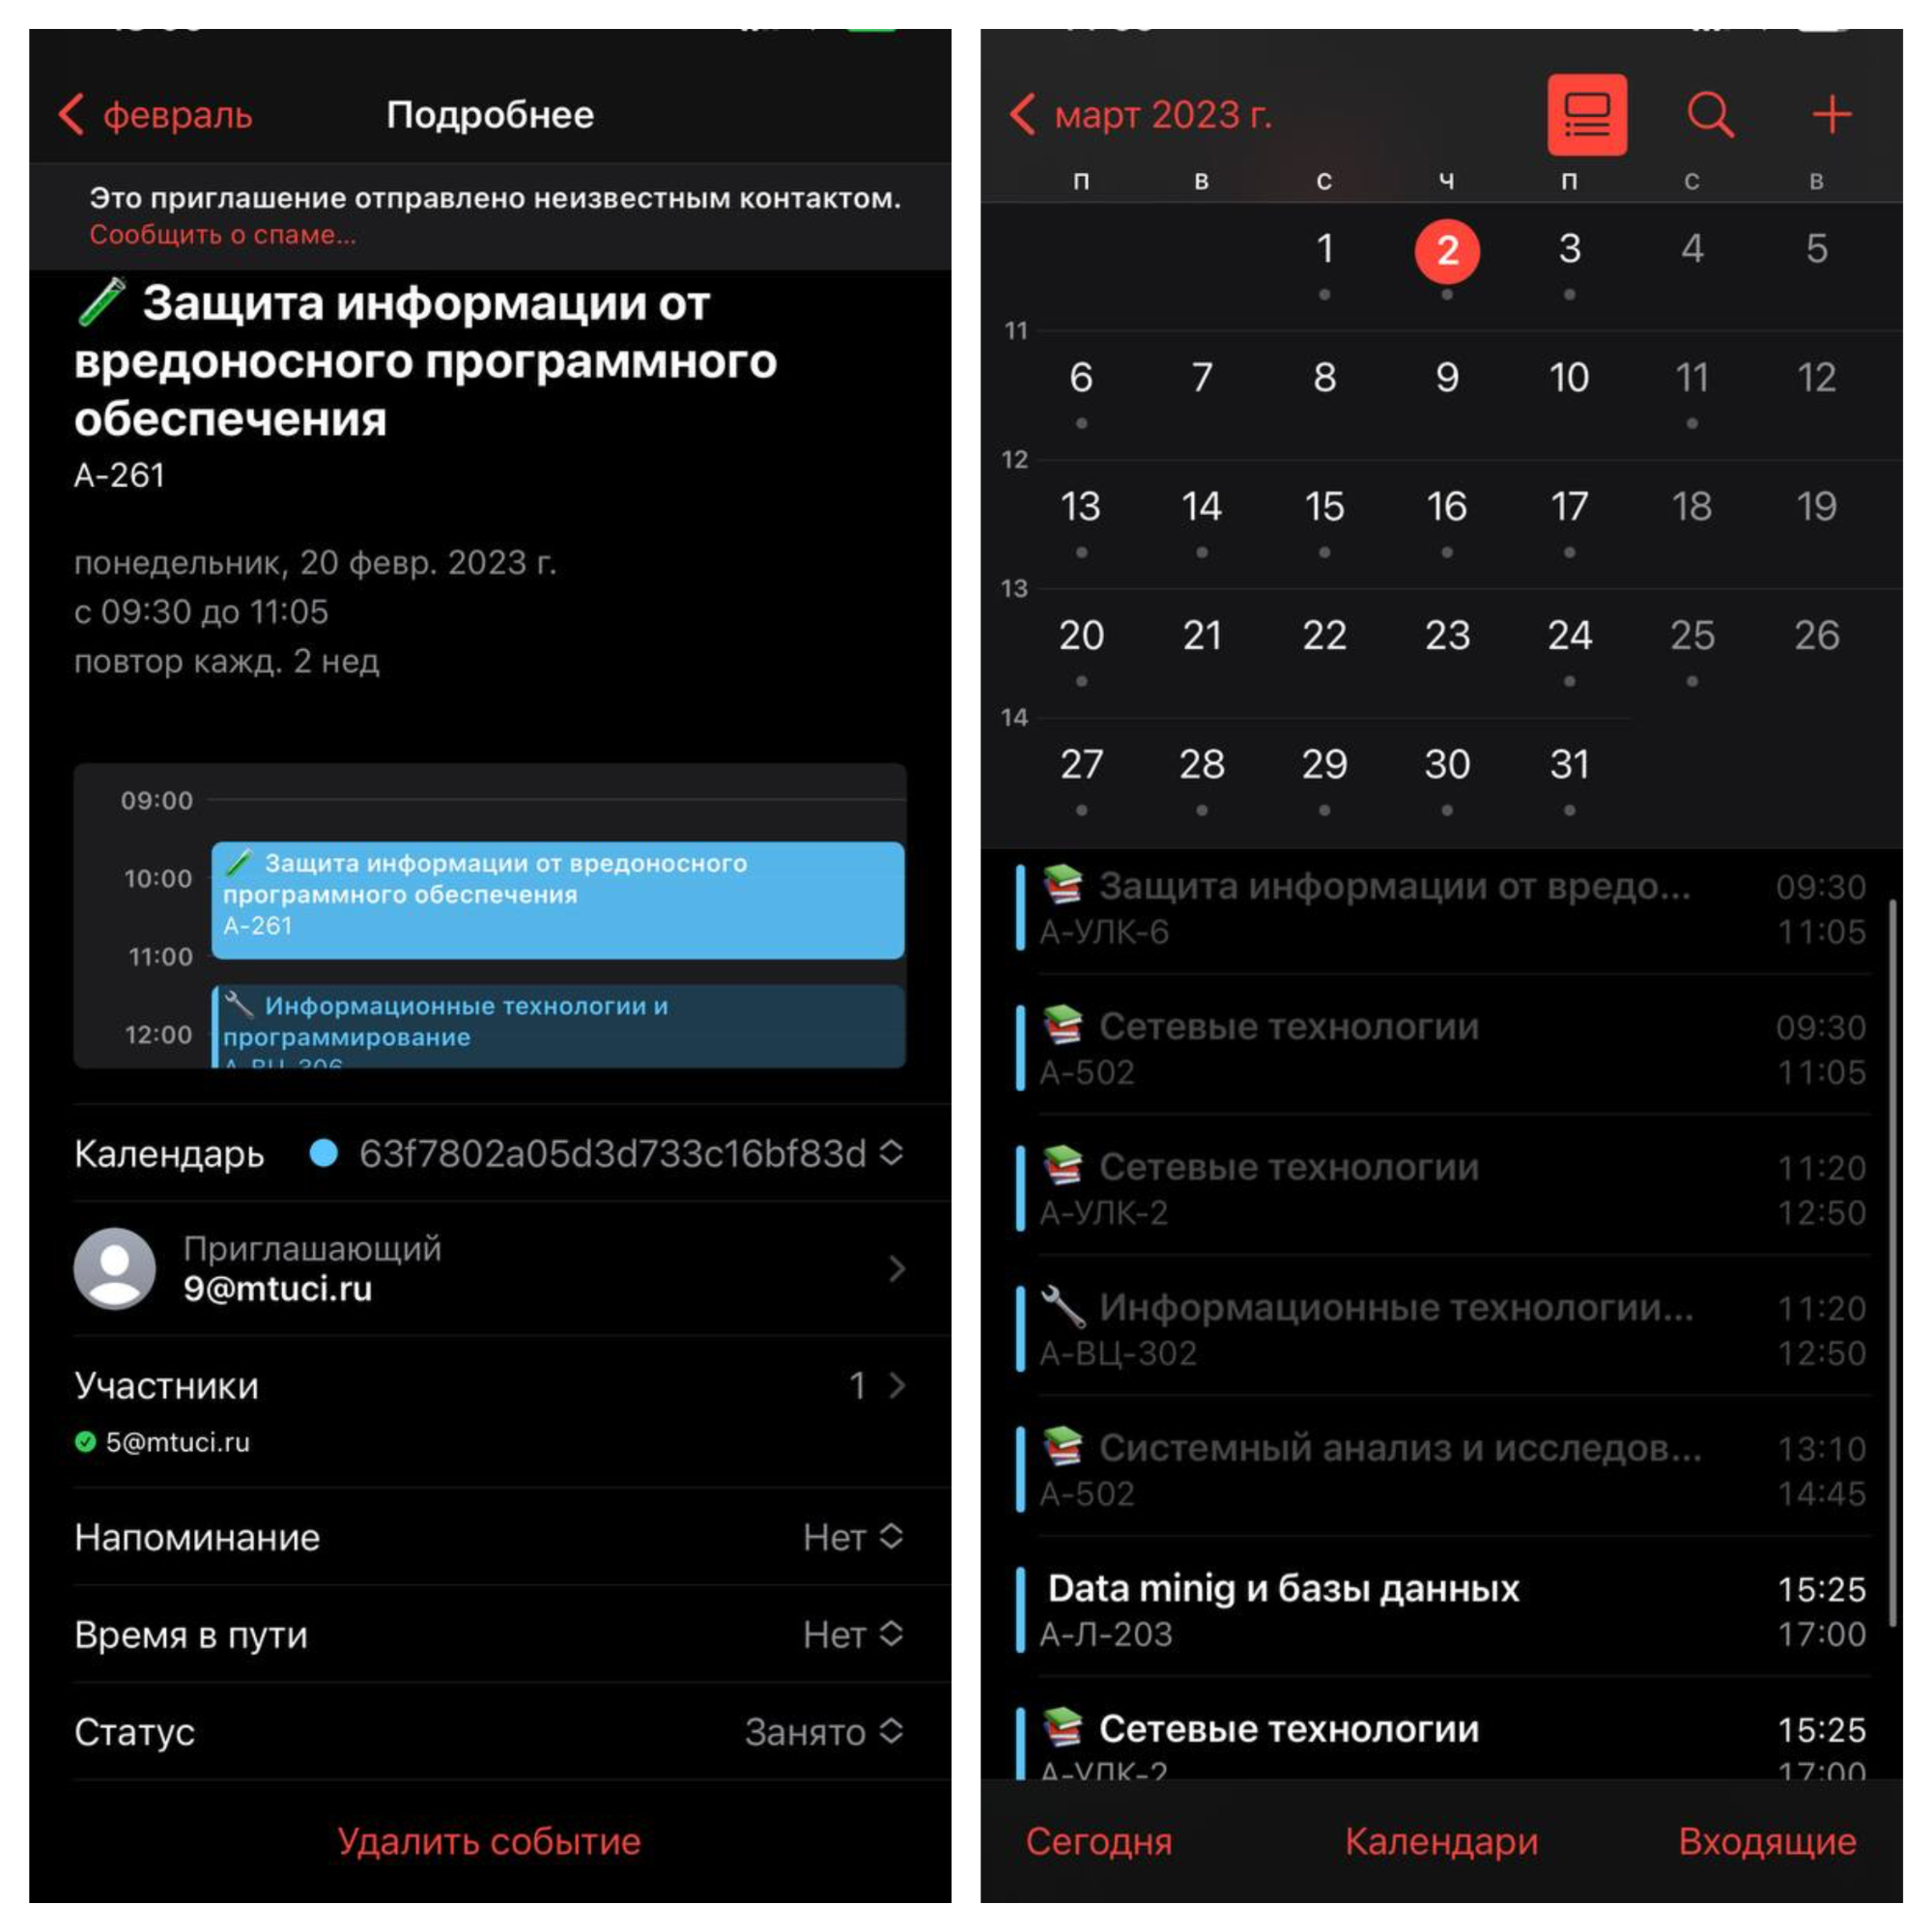
\includegraphics[width=0.8\linewidth]{images/schemes/ics.png}
  \caption{Схема взаимодействий сервиса ICS API. Линии показывают направление передачи данных.}
  \label{fig:schemes:ics}
\end{figure}

Сервис парсера расписания сканирует email-почту, извлекает из нее расписание, помещает его в базу данных.
Схема взаимодействий сервиса парсера расписания представлена на рисунке \ref{fig:schemes:parser}.

\begin{figure}
  \centering
  \includegraphics[width=0.8\linewidth]{images/schemes/parser.png}
  \caption{Схема взаимодействий сервиса парсера расписания. Линии показывают направление передачи данных.}
  \label{fig:schemes:parser}
\end{figure}

Сервис API расписания предоставляет доступ к данным расписания,
полученным из базы данных. Схема взаимодействий сервиса API расписания представлена на рисунке \ref{fig:schemes:api}.

\begin{figure}
  \centering
  \includegraphics[width=0.8\linewidth]{images/schemes/api.png}
  \caption{Схема взаимодей ствий сервиса API расписания. Линии показывают направление передачи данных.}
  \label{fig:schemes:api}
\end{figure}

\section{Технологический стек}

\subsection{Технология БД}
В качестве технологии базы данных (БД) для АИС "Мтуси.Расписание"
была выбрана MongoDB. MongoDB является документоориентированной NoSQL БД,
которая отлично подходит для хранения и
обработки структурированных и полуструктурированных данных.
Она предоставляет гибкую модель данных,
основанную на документах JSON-подобного формата,
что облегчает разработку и интеграцию данных в систему.

Выбор MongoDB обусловлен рядом факторов. Во-первых, она обладает высокой производительностью и масштабируемостью,
что особенно важно для АИС, обрабатывающей большой объем данных расписания и обеспечивающей множество пользователей.
Во-вторых, MongoDB предоставляет богатый набор инструментов и возможностей,
включая гибкий запросов на языке MongoDB Query Language (MQL), и
ндексацию данных для ускорения поиска и агрегации, а также горизонтальное
масштабирование с помощью репликации и шардирования.

Кроме того, MongoDB обладает хорошей поддержкой в популярных языках программирования,
таких как Java, Python, JavaScript и других, что облегчает интеграцию с различными компонентами АИС.
Ее гибкость и простота использования позволяют эффективно работать с изменяющимися
требованиями и структурой данных расписания, что важно для системы,
где расписание может содержать различные типы событий и атрибуты.

Таким образом, MongoDB является оптимальным выбором в
качестве БД для АИС "Мтуси.Расписание", обеспечивая гибкость, производительность
и масштабируемость, необходимые для эффективного хранения и обработки данных расписания.

\subsection{Язык програмирования для серверной части}
Для разработки серверных сервисов в составе АИС "Мтуси.Расписание" был выбран язык программирования Kotlin.
Kotlin является современным языком, разработанным на платформе Java, и обладает рядом преимуществ,
которые делают его идеальным выбором для создания серверных сервисов.

Одним из главных преимуществ Kotlin является его совместимость с Java.
Это позволяет переиспользовать уже существующий Java-код, библиотеки и инструменты, ч
то упрощает интеграцию и расширение функциональности АИС.
Также Kotlin обладает богатым набором стандартных библиотек и инструментов,
что упрощает разработку и ускоряет процесс создания сервисов.

\subsection{Технологии для сервиса API}
Для реализации сервиса API в АИС "Мтуси.Расписание" были выбраны современные технологии, такие как Spring и GraphQL.

Spring является одним из наиболее популярных фреймворков для разработки серверных приложений на Java.
Он предоставляет широкий набор инструментов и компонентов, которые значительно упрощают разработку,
развертывание и масштабирование сервисов API. Spring обладает мощной системой управления зависимостями,
интегрированным контейнером внедрения зависимостей и механизмами обработки запросов,
что делает разработку API быстрой и эффективной. Кроме того,
Spring предоставляет инструменты для обработки запросов и ответов, управления сеансами пользователя и обеспечения безопасности данных.

GraphQL -- это современный язык запросов и среда выполнения запросов для API.
В отличие от традиционного подхода REST API, который возвращает фиксированную структуру данных,
GraphQL позволяет клиентам запрашивать только необходимые данные,
уменьшая избыточность и улучшая производительность.
GraphQL также обладает гибкостью и возможностью составлять сложные запросы, объединяя данные из различных источников.
Это особенно полезно в АИС "Мтуси.Расписание", где клиентское приложение может требовать
различные данные о расписании в зависимости от своих потребностей.

Использование Spring и GraphQL в сервисе API позволяет создавать эффективные,
гибкие и масштабируемые интерфейсы, обеспечивающие удобство использования и
оптимальное взаимодействие между клиентскими приложениями и серверной частью АИС "Мтуси.Расписание".

\subsection{Технологии для сервиса парсера расписания}
Для реализации сервиса парсера расписания в АИС "Мтуси.Расписание" были выбраны технологии Apache POI и JSOUP.

Apache POI - это библиотека для работы с форматами файлов Microsoft Office,
такими как Excel, Word и PowerPoint. Она предоставляет набор классов и методов для чтения,
записи и манипуляции данными в этих форматах. В контексте парсера расписания,
Apache POI может использоваться для извлечения данных из файлов Excel,
содержащих расписание занятий, экзаменов и других событий.
Благодаря Apache POI, сервис парсера может эффективно обрабатывать и преобразовывать
данные из Excel-файлов в удобный формат для дальнейшей обработки и предоставления через API.

JSOUP - это Java-библиотека для парсинга HTML и XML-документов.
Она обладает простым и интуитивно понятным API, позволяющим извлекать информацию из веб-страниц и документов
с помощью CSS-подобного синтаксиса. В контексте парсера расписания, JSOUP может использоваться для извлечения данных из HTML-страниц,
содержащих расписание, а также для навигации по DOM-дереву и поиска необходимых элементов.
JSOUP обеспечивает гибкость и удобство в работе с HTML-документами, что
позволяет сервису парсера эффективно извлекать и структурировать данные из веб-страниц.

Использование Apache POI и JSOUP в сервисе парсера расписания обеспечивает
надежные и мощные инструменты для обработки и извлечения данных из файлов Excel и HTML-страниц.
Это позволяет сервису парсера эффективно обрабатывать различные источники данных с расписанием и преобразовывать их
в единый формат для дальнейшей обработки и предоставления через API.

\subsection{Технологии для сервиса ICS API}
Для реализации сервиса ICS API в АИС "Мтуси.Расписание" были выбраны технологии ktor и Amazon S3.

ktor - это асинхронный фреймворк для разработки серверных приложений на языке Kotlin.
Он предоставляет удобные средства для создания API и обработки HTTP-запросов.
ktor обладает простым и выразительным синтаксисом, позволяющим быстро создавать маршруты,
обрабатывать запросы и формировать ответы. Благодаря своей асинхронной природе,
ktor обеспечивает высокую производительность и масштабируемость при обработке запросов в сервисе ICS API.
Кроме того, ktor обладает интеграцией с различными модулями и расширениями, что позволяет легко взаимодействовать
с другими сервисами и инструментами.

Amazon S3 (Simple Storage Service) - это облачное хранилище данных, предоставляемое Amazon Web Services (AWS).
Оно предоставляет надежное и масштабируемое хранилище файлов, которое может использоваться для кеширования данных в сервисе ICS API.
Amazon S3 позволяет сохранять и получать файлы любого размера и формата,
обеспечивая высокую доступность и низкую задержку при получении данных.
Использование Amazon S3 для кеширования данных позволяет сервису ICS API эффективно управлять большим
объемом данных и ускорить доставку расписания клиентским приложениям.

Сочетание ktor и Amazon S3 обеспечивает надежность, производительность и масштабируемость в сервисе ICS API.
ktor обеспечивает быструю и эффективную обработку запросов, а Amazon S3 предоставляет надежное хранилище данных для кеширования.
Такой технологический стек позволяет создать мощный и надежный сервис ICS API для экспорта расписания в формате iCalendar.

\subsection{Технологии для мобильного приложения}

Для разработки мобильного приложения в АИС "Мтуси.Расписание" были выбраны следующие технологии: Flutter, Riverpod и Dio.

Flutter - это фреймворк от компании Google для разработки кросс-платформенных мобильных приложений.
Он позволяет создавать высокопроизводительные и красиво оформленные приложения с использованием единого кодовой базы.
Flutter использует язык программирования Dart, который обладает простым синтаксисом и мощными возможностями.
Он также предоставляет множество готовых виджетов и инструментов для построения пользовательского интерфейса
и взаимодействия с серверной частью. Благодаря своей кросс-платформенной природе,
Flutter позволяет разработчикам создавать приложения, работающие как на iOS, так и на Android.

Riverpod - это библиотека управления состоянием для приложений Flutter.
Она предоставляет удобные инструменты для организации и управления состоянием приложения,
а также обеспечивает инверсию управления зависимостями.
Riverpod основан на принципах "провайдеров" (providers) и "потребителей" (consumers),
что делает код более модульным, расширяемым и тестируемым. Благодаря Riverpod,
разработчики могут эффективно управлять состоянием и зависимостями в мобильном приложении,
что способствует лучшей организации и поддерживаемости кода.

Dio - это мощная и простая в использовании библиотека HTTP-клиента для Dart и Flutter.
Она предоставляет инструменты для выполнения HTTP-запросов и обработки ответов от сервера.
Dio поддерживает различные функции, такие как аутентификация, отправка файлов,
управление заголовками запросов и др. Благодаря Dio, разработчики могут легко взаимодействовать
с API расписания и получать необходимые данные из серверной части.
Он обладает удобным API и интегрируется хорошо с другими компонентами Flutter-приложения.

Использование Flutter, Riverpod и Dio в мобильном приложении обеспечивает быструю разработку,
эффективное управление состоянием и легкость взаимодействия с серверной частью.
Такой технологический стек позволяет создать мощное и удобное мобильное приложение для просмотра расписания в АИС "Мтуси.Расписание".
